
\documentclass[a4paper,12pt]{article} % тип документа


% Русский язык
\usepackage[utf8]{inputenc}
\usepackage[russian]{babel}
\usepackage[OT1]{fontenc}
\usepackage{amsmath}
\usepackage{amsfonts}
\usepackage{amssymb}
\usepackage{graphicx}
\graphicspath{{images/}}
\usepackage{wrapfig}
\usepackage[left=2cm,right=2cm,top=2cm,bottom=2cm]{geometry}
\usepackage{setspace}
\DeclareGraphicsExtensions{.pdf,.png,.jpg}


% Математика
\usepackage{amsmath,amsfonts,amssymb,amsthm,mathtools}


\usepackage{wasysym}

%Заговолок
\author{Талашкевич Даниил Александрович}

\title{Лабораторная работа 1.2.3}

\date{\today}

\begin{document}

\maketitle
\thispagestyle{empty}

\newpage
\setcounter{page}{1}


{\bf 1. Аннотация}

В данной работе мы будем измерять момент инерции ряда тел и сравнивать результаты с расчетами по теоретическим формулам; проверка аддитивности моментов инерции и справедливости формулы Гюйгенса-Штейнера.

{\bf 2. Используемое оборудование}

Трифилярный подвес, секундомер, счетчик числа колебаний, набор тел, момент инерции которых надлежит измерить(диск, стержень, полый цилиндр и другие).

{\bf 3. Теоретические сведения}

Инерционность вращения тела относительно оси определяется моментом инерции тела отностильно этой оси(см. введегние к данному разделу). Момент инерции твердого тела относительно неподвижной оси вращения вычисляется по формуле 
\[ I = \int r^2 dm .\]

Здесь $r$ -- расстояние элемента массы тела $dm$ от оси вращения. Интегрирование проводится по всей массе тела $m$. 

\begin{center}
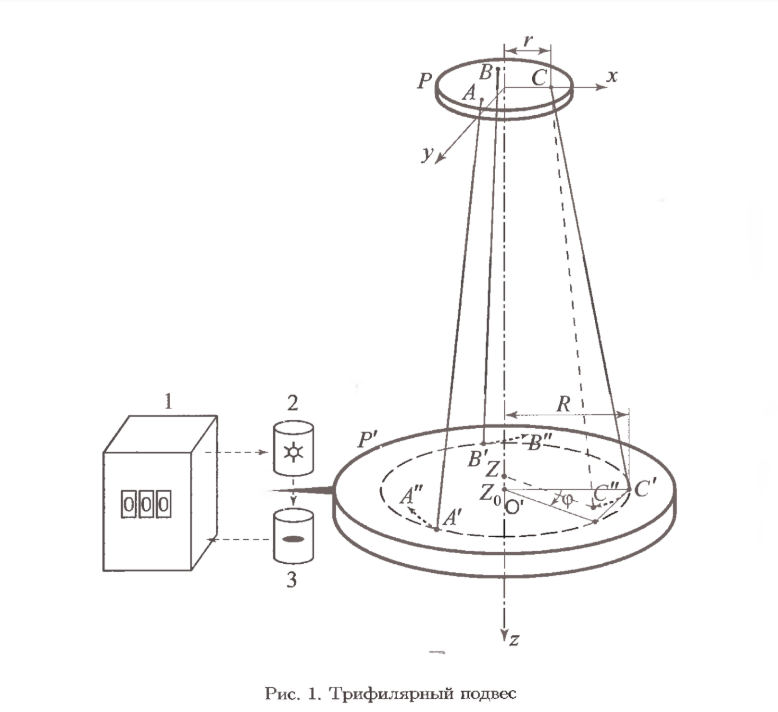
\includegraphics[scale=0.6]{1.2.3 1}
\end{center}

Для однородных тел известной плотности при заданных размерах и достаточно простой форме момент инерции можно вычислить. Для неоднородных тел и тел сложной формы момент инерции можно определить экспериментально. Удобно использовать устройство, показаное на рис. 1 и называемое трифилярным подвесом. Оно состоит из вешенной к ней на трех симметрично расположенных нитях $AA^{'}$, $BB^{'}$ и $CC^{'}$ вращающейся платформы $P^{'}$.

Платформа $P$ укреплена на кронштейне и снабжена рычагом (на рисунке не показан), при помощи которого в системе можно создать крутильные колебания путем небольшого поворота верхней платформы. Лучше поворачивать верхнюю платформу, укрепленную на неподвижной оси, чем подвешенную на нитях нижнюю, так как нижнюю платформу трудно закрутить не вызвав ее раскачиваний, подобных движению маятника, учет которыъ сильно усложнил бы расчеты. После поворота, вызывающего крутильные колебания, верхняя платформа остается неподвижной в течение всего процесса колебаний. После того, как нижняя платформа $P^{'}$ оказывается повернутой на угол $\varphi$ относительно верхней платформы $P$, возникает момент сил, стремящийся вернуть нижнюю платформу в положение равновесия, при котором относительный поворот платформ отсутствует. Но в положении равновесия платформа не останавливается, так как имеет угловую скорость(кинетическую энергию вращения). В результате платформа совершает крутильные колебания.

Если пренебречь потерями энергии на трение(о воздух и в креплениях нитей), то уравнение сохранения энергии при колебаниях можно записать следующим образом:
\[ \frac{I \dot{\varphi^2}}{2}\]

Здесь $I$ -- момент инерции платформы вместе с исследуемым телом, $m$ -- масса платформы с телом, $\varphi$ -- угол повороты платформы от положения равновесия системы, точкой обозначена производная по времени (угловая скорость), $z_0$ -- координата по вертикали центра нижней платформы $O^{'}$ при равновесии ($\varphi = 0$), $z$ -- координата той же точки при некотором угле поворота $\varphi$. Первый член в левой части уравнения -- кинетическая энергия вращения, второй член -- потенциальная энергия в поле тяжести, $E$ -- полная энергия системы (платформы с тулом).

Отметим, что, как показывает соотношения (2), возвращающая сила возникает благодаря силе тяжести.

Воспользуемся системой координат $x,y,z$ связанной с верхней платформой, как показано на рис. 1. Координаты верхнего конца одной из нитей подвеса точки $C$ в 
этой системе -- $(r, 0, 0)$. Нижний конец данной нити $c^{'}$, находящейся на нижней платформе, при равновесии иметт координаты ($R,0,z_0$), а при повороте платформы на угол $\varphi$ эта точка переходит в $C^{''}$ с координатами ($R \cos{\varphi}, R\sin{\varphi},z$). Расстояние между точками $C^{'}$ и $C^{''}$ равно длине нити $L$. Поэтому 
\[ (R\cos{\varphi} - r)^2 +R^2\sin^2{\varphi} +z^2 = L^2 .\]

Учитывая, что при малых углах поворота $\cos{\varphi} \approx 1 -\frac{\varphi^2}{2}$, получаем 
\[ z^2 = L^2 - R^2 - r^2 +2Rr\cos{\varphi} = z_0^2 - 2Rr(1 - \cos{\varphi})\approx z_0^2 - Rr\varphi^2 .\]

Извлекая из выражения выше квадратный корень и учитывая малость угла $\varphi$, имеем 
\[ z \approx \sqrt{z_0^2 - Rr\varphi^2}\approx \sqrt{1-\frac{Rr\varphi^2}{z_0^2}}\approx z_0 = \frac{Rr-varphi^2}{2z_0} .\]

Подставляя это значение $z$ в уравнение сохранения энергии получаем 
\[ \frac{1}{2}I \ddot{\varphi} + mg\frac{Rr}{z_0}\varphi = 0.\] 

Производная по времени от $E$ равна нулю, так как потерями энергии на трение, как уже был сказано выше, пренебрегаем.

Решение этого уравнения, как нетрудно убедиться простой подстановкой, имеет вид 
\[ \varphi = \varphi_0\sin{\sqrt{\frac{mgRr}{Iz_0}}t + \Theta} .\]

Здесь амплитуда $\varphi_0$ и физа $\Theta$ колебаний определяются начальными условиями. Период крутильных колебаний нашей системы равен 
\[ T = 2\pi \sqrt{\frac{Iz_0}{mgRr}}.\]

Обратим внимание на то, что из этой формулы при $r = R$ и $I = mR^2$ (тонкое кольцо) получаем формулу для математического маятника. Из последнего уравнения находим формулу для определения момента инерции:
\[ I = \frac{mgRrT^2}{4\pi^2 z_0}.\]

Учитывая, что параметры установки $R,r$ и $z_0$ при проведении опытов не меняются, удобно переписать последнее уравнение следующим образом: 
\[ I = kmT^2.\]

Здесь $k = \frac{gRr}{4\pi^2 z_0}$ -- величина, постоянная для данной установки.

Таким образом, полученные формулы позволяют определить момент инерции платформы с телом и отдельно платформы по соответствующим периодам крутильных колебаний. Затем вычисляем момент инерции тела, пользуясь аддитивностью, в справедливости которой можно убедиться, проведя измерения сначала для каждого из двух тел отдельно, а затем для обоих тел вместе.

При выводе формул предполагалось, что малы необратимые потери энергии, связанные с трением, то есть мало затухание колебаний. О затухании колебаний можно судить, сравнивая время $\tau$ уменьшения амплитуда колебаний в 2-3 раза с периодом колебаний $T$. Необратимыми потерями энергии можно пренебречь, если выполняется условие 
\[ \tau \gg T .\]

В данной работе рекомендуется период клебаний определять с относительно погрешностью $0.5\%$. Число колебаний, по которым надо вычислять период, определяется этой погрешностью и погрешностью ихмеоения времени.

Для счета числа колебаний используется счетчик, состоящий из осветителя(2), фотоэлемента (3) и пересчетного устройства (1) (см. рис.1). Легкий лепесток, укрепленный на платформе, при колебаниях пересекает световой луч дважды за период. Соответствующие сигналы от фотоэлемента поступают на пересчетное устройство.

\begin{center}
{\bf ХОД РАБОТЫ}
\end{center}
{\bf Характеристики установки и таблицы полученных данных}

Константы установки: $z_0 = 2.14 \pm (5\cdot 10^{-5})$ м; $m = 1012.5 \pm 0.5$ гр; $R = 114.6 \pm 0.5$ мм; $r = 30.5 \pm 0.3$ мм; $T = 4.46$ с; $\Rightarrow k = \frac{gRr}{4\pi^2 z_0} = 4.14\cdot 10^{-4}$.

Таблицы полученных данных:

\begin{center}
\begin{tabular}{|c|c|c|c|}
\hline 
$20T$ & $75.354$ & $85.428$ & $73.763$\\ 
\hline 
$T$ & $3.768$ & $4.271$ & $3.688$ \\ 
\hline 
$N_{\textbf{тела}}$ & $1$ & $2$ & $3$\\ 
\hline 
\end{tabular} 
\end{center}

Здесь тело 1 -- это брусок, 2 -- кольцо, а 3 -- диск.

Для тела $2$ и $3$ совмещенные вместе получили $20T = 74.21$, $T = 3.711$.

Таблица для пункта 7:
\begin{center}
\begin{tabular}{|c|c|c|c|c|c|c|c|c|}
\hline 
$20T$, c & 62.913 & 63.182 & 63.392 & 63.712 & 64.383 & 66.193 & 67.231 & 68.242\\ 
\hline 
$T$, c & 3.146 & 3.160 & 3.170 & 3.186 & 3.219 & 3.310 & 3.362 & 3.412\\ 
\hline 
$h$, м$\cdot 10^{-2}$ & 0 & 1 & 2 & 3 & 4 & 5 & 6 & 7\\ 
\hline 
$I$, кг$\cdot$м$^2\cdot 10^{-3}$       & 10.603 & 10.697 & 10.765 & 10.874 & 11.101 & 11.5 & 12.109 & 12.472\\ 
\hline 
$h^2$, м$^2\cdot 10^{-4}$ & 0 & 1 & 4 & 9 & 16 & 25 & 36 & 49\\ 
\hline 
\end{tabular} 
\end{center}

\begin{center}
\begin{tabular}{|c|c|c|c|}
\hline
$20T$, c                  & 69.744 & 71.414 & 74.137\\ 
\hline 
$T$,   c                  & 3.487 & 3.571 & 3.707\\ 
\hline 
$h$, м$\cdot 10^{-2}$     & 8 & 9 & 10\\ 
\hline 
$I$, кг$\cdot$м$^2\cdot 10^{-3}$  & 13.026 & 13.661 & 14.721\\ 
\hline 
$h^2$, м$^2\cdot 10^{-4}$ & 64 & 81 & 100\\ 
\hline
\end{tabular}
\end{center}






{\bf $1$. Проверка установки} 

Сначала проверим, пригодна ли установка для измерений, то есть нормально ли функционирует устройство для возбуждения крутильных колебаний, не возникают ли при этом нежелательные маятниковообразные движения, работает ли счетчик числа колебаний.

Устроцство для возбуждения крутильных колебаний функционирует нормально, нежелательных маятниковообразных движений не возникает, счетчик числа колебаний работает нормально.

{\bf $2$. Проверка затухания колебаний.}

Сравним время $\tau$ уменьшения амплитуды колебаний в $2-3$ раза с периодом колебаний $T$. Получили, что выполняется соотношение $\tau \gg T.$

Для удобства наблюдения, определим, за каrое время амплитуда колебаний платформы (угол $\alpha$ - угол отклонения от начального положения) уменьшиться в 2 раза.
		
Для значения $\alpha \approx 45^{\circ}$ имеем: Время затухания: $\tau \approx 180$ секунд, $T \approx 1,5$ секунды. Соотношение выполняется, установка пригодна для проведения измерений. Кроме того, определим, при каком значении угла отклонения амплитуда практически независит от периода. Путем измерений начальное отклонение было выбрано $\alpha' \approx 30^{\circ}$

{\bf $3$. Рабочий диапазон амплитуд}

Найдем рабочий диапазон амплитуд колебаний. Амплитуду будем уменьшать до тех пор, пока период колебаний, определенный по $20-30$ полным колебаний, не перестанет зависеть от амплитуды. Рабочий диапазон будет начинаться с тех амплитуд, для которых период совпадает с периодом колебаний амплитуд вдвое меньше.

{\bf $4$. Параметры установки}

Измеряем параметры установки $z_0, R, r$ (см. рис. 1). По ним вычисляем константу установки $k$, входящую в формулу $(11)$, и ее погрешность $\sigma_k.$

\[ k = \frac{gRr}{4\pi^2z_0} \approx 4.14\cdot10^{-4}.\] 
$$ \sigma_k = \sqrt{(\frac{\sigma k}{\sigma R})^2\cdot\sigma_R^2 + (\frac{\sigma k}{\sigma r})^2\cdot \sigma_r^2 + (\frac{\sigma k}{\sigma z_0})^2\cdot \sigma_{z_0}^2} = \sqrt{ (\frac{gr}{4\pi^2z_0})^2\cdot \sigma_R^2 + (\frac{gR}{4\pi^2z_0})^2\cdot \sigma_r^2 +  (\frac{gRr}{4\pi^2 z_0^2})^2\cdot \sigma_{z_0}^2} = 0.06\cdot 10^{-4}.$$

Значит $k = (4.14\pm 0.06)\cdot 10^{-4}$ .

{\bf $5$. Определение моментра инерции}

Определяем момент инерции ненагруженной платформы (здесь и далее периоды колебаний мы будем определять с относительной погрешностью не хуже $0.5\%$).

Для определения момента инерции установки возбудим крутильные колебания ненагруженной платформы. Измерим период колебаний ненагруженной платформы. Для этого измерим время $N$ полных колебаний установки. По результатам измерений определим $ T_{0} = \frac{t_N}{N}$.
		
Результаты измерений: $ N = 50,\ \langle t_{N} \rangle= 223,054$ cекунд, $\langle T_{0} \rangle = 4,46$ c. $\sigma_{T_0} = 0.0009$ c.  

Получаем момент инерции ненагруженной платформы $I_0 = (8.34\pm 0.11)\cdot 10^{-3}$ кг$\cdot$м$^2$.

{\bf $6$. Измерение момента инерции различных тел}

Измеряем моменты инерции различных тел из имеющегося набора. Сначала порознь,а затем вместе. Помещать тела на платформу будем там, чтобы общий центр масс всегда находился на оси вращения (оси симметрии) системы, то есть чтобы не было заметного перекоса платформы. По полученным данным проверяем аддитивность моментов инерции, то есть справедливость соотношения $I = I_1 + I_2$, где $I_1$ и $I_2$ -- моменты инерции первого и второго тел, а $I$ -- общий момент инерции. Погрешность, с которой выполняется это соотношение, является хорошей мерой точности проводимых измерений. Так же рассчитаем теоритически моменты инерции $I$ всех используемых в эксперименте тел и сравним результаты с измеренными экспериментально значениями $I$.

Определив период колебаний свободной платформы, можно перейти к определению периодов колебаний подвеса с грузами, установленными на платформе. Результаты измерений заносим в таблицу \ref{tab:periods_diff_body}.
		
\begin{table}[ht!]
\begin{center}
\begin{tabular}{| p{65pt} | p{65pt} | p{55pt} | p{60pt}  | p{60pt} |}
					\hline
					Тело & Количество колебаний & Время колебаний, с & Период колебаний, с & Масса груза, г \\ \hline
					платформа & 50 & 223.054 & 4,46 & 1012 \\ \hline
					платформа, кольцо & 20 & 85.428 & 4.271 & 1760 \\ \hline
					платформа, диск & 20 & 73.763 & 3.688 & 1520 \\ \hline
					платформа, кольцо, диск & 20 & 74.21 & 3,711 & 2268 \\
					\hline
\end{tabular}
\end{center} 
\caption{Периоды колебаний для различных тел на трифилярном подвесе.}
\label{tab:periods_diff_body}
\end{table}
		
		Для подтверждения аддитивности момента инерции необходимо показать, что выболняются соотношение:
		$$ I_{ring + disc} = I_{ring} + I_{disc} - I_{0} $$
		
		Для подтверждения данного соотношения вычислим соответсвующие моменты инерции, используя формулу для нахождения моментов инерции. Результаты занесем в таблицу ($\ref{tab:moments}$)
		
\begin{table}[h!]
\begin{center}
\begin{tabular}{| l | c |}
				\hline
				Тело & Момент инерции, $kg*m^{2}, * 10^{-3}$ \\ \hline
				Платформа & 8.33 \\ \hline
				Платформа + диск & 13.3 \\ \hline
				Платформа + кольцо & 8.56 \\ \hline
				Платформа + диск + кольцо & 12.9 \\ \hline
\end{tabular}
\caption{Моменты инерции различных тел.}
\label{tab:moments}
\end{center}					
\end{table}

Теоретические значения моментов инерции будем рассчитывать по разным формулам для разных тел. Для кольца $I = mr^2$, для бруска $I = \frac{ml^2}{12}$, для диска $I = \frac{mr^2}{2}$.
		
		Подставляя эти данные в формулу $$ I_{ring + disc} = I_{ring} + I_{disc} - I_{0}, $$ получаем, что данное соотношение выполняется в пределах погрешности. Значит, доказано исходное предположение, \underline{момент инерции тела -- аддитивная величина}.

Так же рассчитаем погрешность для измерения момента инерции: 

\[ 	 \]


{\bf 7. Определение зависимости момента инерции системы тел от их взаимного расположения.}

Поместим на платформу диск, разрезанный по диаметру. Постепенно раздвигая половинки диска так, чтобы их общий центр масс все время оставался на оси вращения платфомры (рис. 2), снимаем зависимость момента инерции такой системы $I$ от расстояния $h$ каждой из половинок до оси вращения (центра платформы).

Строим график полученной зависимость $I(h^2)$ и определим по нему массу и момент инерции диска.

\begin{wrapfigure}[10]{r}{0.29\textwidth}
\vspace{-3em}
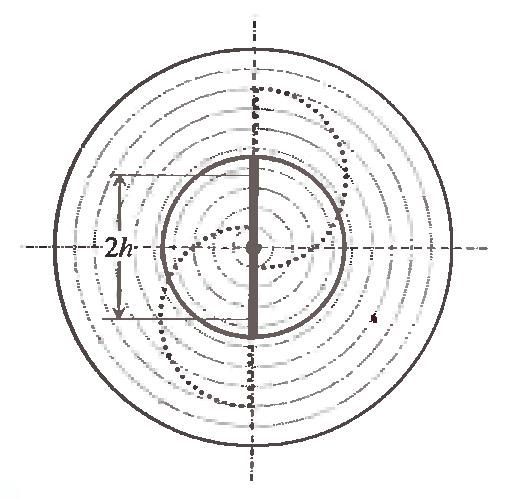
\includegraphics[width=0.25\textwidth]{position}
\caption{Схема расположения грузов на платформе трифилярного подвеса.}
\label{ris:position}
\end{wrapfigure}
			
Перейдем к определению зависимости Момента инерции системы двух тел от их взаимного расположения. Для этого, располагая грузы как показано на рис. \ref{ris:position}, получим зависимость периода от расстояния. Затем, используя формулу для нахождения момента инерции, определим зависимость $ I(h^{2}) $
	
Полученные результаты измерений занесем в таблицы  соответсвенно. Основывыаясь на результатах таблицы вначале, построим график зависимости $ I(h^{2}) $. (Рис. \ref{ris:grafik})
		
Таблица зависимости момента инерции от $h^2$:



		
\begin{center}
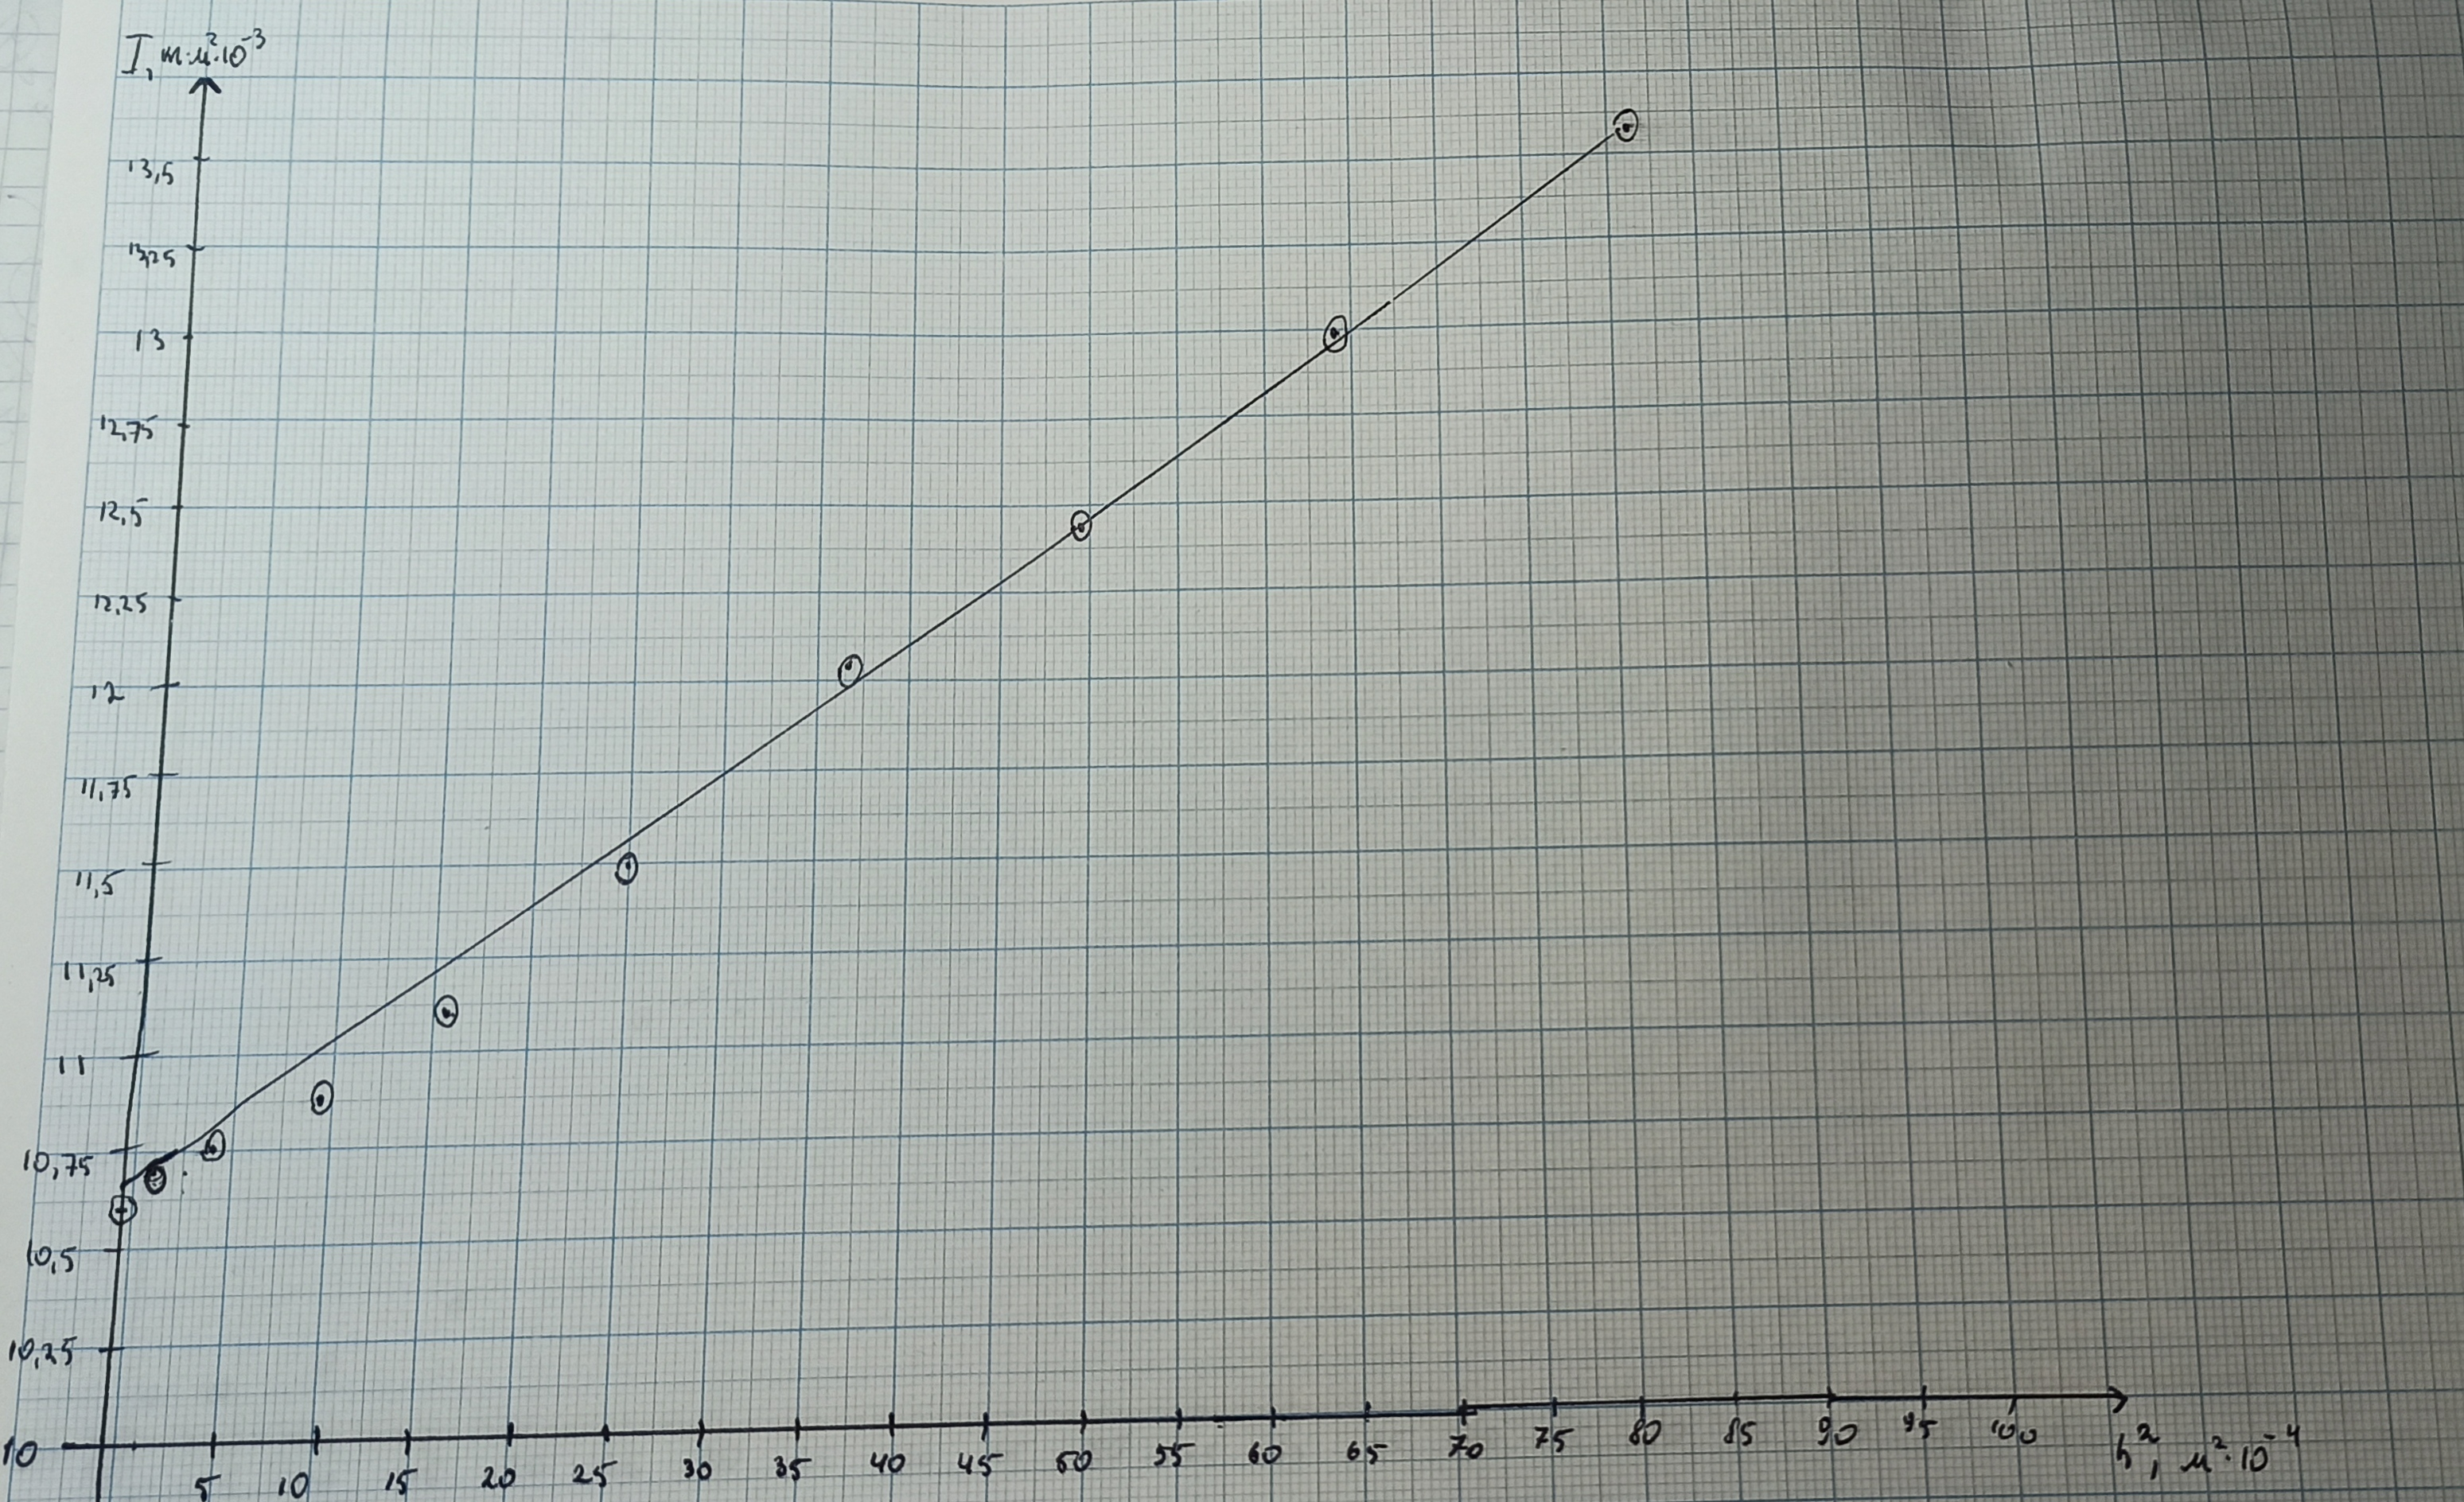
\includegraphics[width=0.9\textwidth]{3}
\label{ris:grafik}
\end{center}

{\bf Вывод : }
\begin{enumerate}
		\item Величина момента инерции, определенная с помощью трифилярного подвеса с довольно большой точностью совпадает с теоретическими предсказаниями. Большая точность обеспечивается малой погрешностью измерения времени, а также выбором условий, при которых крутильные колебания подвеса можно считать слабозатухающими.
		\item Была достигнута относительная точность определения момента инерции $ \epsilon_{I} = 0,089 $. Основной вклад в погрешность измерения момента инерции внесла погрешность косвенного измерения $z_{0}$. Данную погрешность можно уменьшить, если более точно определить параметры установки.
		\item Была полученая зависимость $ I(h^{2}) $. Данная зависимость довольно хорошо аппроксимируется линейной зависимость, что подтверждает теоретические данные.
		\item Была подтверждена аддитивность момента инерции.
	\end{enumerate}










${\bf }$









\end{document}


